\begin{frame}{Sunflowers [Erd\H{o}s, Rado 60; Rossman 14]}

    \begin{minipage}{0.55\linewidth}
        $(k, \ell)$-sunflower:
        \begin{itemize}
            \item $S_1, S_2, S_3, \dots, S_{\ell} \subseteq \{0, 1\}^n$ of size $k$;
            \item $Z \coloneqq \bigcap S_i$;
            \item $\forall i, j ~~~ S_i \cap S_j = Z$.
        \end{itemize}
    \end{minipage}
    \begin{minipage}{0.2\linewidth}
        \centering
        \pause
        
\begin{tikzpicture}

    \foreach \i in {0, 40, ..., 330}{
        \begin{scope}[rotate = \i]
            \draw[fill = yellow!80!black] (0, 0) to[out = 75, in = 0] (0, 1) to[out = 180, in = 105]
                cycle;
        \end{scope}
    }
    
    \node[circle, fill = yellow!40!black, draw, inner sep = 0, minimum size = 0.5cm] at (0, 0)
        {\textcolor{blue}{$Z$}};
\end{tikzpicture}
    \end{minipage}
    \begin{minipage}{0.2\linewidth}
        \centering
        \pause
        \includegraphics[scale = 0.1]{pics/cagney.png}
    \end{minipage}

    \pause
    \vspace{0.3cm}
    
    \begin{minipage}{0.55\linewidth}
        $(p, \varepsilon)$-robust sunflower:
        \begin{itemize}
            \item $S_1, S_2, S_3, \dots \subseteq \{0, 1\}^n$ of size $k$;
            \item $Z \coloneqq \bigcap S_i$;
            \item $\Pr\limits_{W \sim \mathbf{U}_p}[\exists i, W \subseteq (S_i \setminus Z)] \ge 1 -
                \varepsilon$.
        \end{itemize}
    \end{minipage}
    \begin{minipage}{0.4\linewidth}
        \centering
        \pause
        \includegraphics[scale = 0.1]{pics/cagney2.png}
    \end{minipage}

    \pause
    \begin{block}{}
        Every $\left( 1 / \ell, 1 / \ell\right)$ robust sunflower contains a sunflower with
        $\ell$ petals.
    \end{block}
\end{frame}


\begin{frame}{Clique vs. Monotone ckt [Razborov 85; Cavalar, Kumar, Rossman 22]}

    \begin{center}
        \begin{tikzpicture}[>=latex]
    \only<1-2>{
        \node[draw, circle, inner sep = 0, minimum size = 0.7cm] (b) at (3.5, -2) {$\lor$};
        
        \foreach \i in {1, 2, ..., 6}{
            \node[draw, circle, inner sep = 0, minimum size = 0.7cm] (a\i) at (\i, 0) {$\land$};
            \draw[->] (a\i) -- (b);
        }
    }
    \only<3->{
        \node[draw, circle, inner sep = 0, minimum size = 0.7cm] (b) at (4.5, -2) {$\lor$};
        
        \foreach \i in {1, 2, ..., 8}{
            \node[draw, circle, inner sep = 0, minimum size = 0.7cm] (a\i) at (\i, 0) {$\mathds{1}_{C_\i}$};
            \draw[->] (a\i) -- (b);
        }
    }

    \draw[->] (b) -- ++(0, -0.7);
\end{tikzpicture}        
    \end{center}


    \pause
    \begin{itemize}
        \item \textsc{No}: $\mathbf{G}_{n, p}$, whp there is no $r$-clique;
            \pause
        \item Approximation of gates via $\bigvee\limits_{j = 1}^{m} \mathds{1}_{C_j}$.
        \item Size of $C_j$ at most $k$ (whp $\mathbf{G}_{n, p}$ has an $n^{\varepsilon} k$-clique).
    \end{itemize}
\end{frame}


\begin{frame}{\textsc{No}: $\mathbf{G}_{n, p}$}

    \begin{center}
        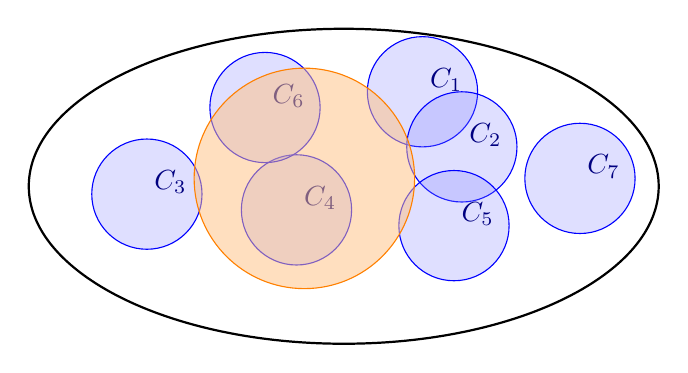
\begin{tikzpicture}
    \def\r{0.7}
    \def\vars{(1, 1.2), (1.5, 0.5), (-2.5, -0.1), (-0.6, -0.3), (1.4, -0.5), (-1, 1), (3, 0.1)}
    
    \draw[thick] (0, 0) ellipse (4 and 2);

    \foreach \a  [count = \i] in \vars{
        \draw[blue, fill = blue!50, fill opacity = 0.25] \a circle (0.7) ++(0.3, 0.15)
            node[opacity = 1, blue!50!black] {$C_{\i}$};
    }
        
    \only<3->{
        \draw[orange, fill = orange!50, fill opacity = 0.5] (-0.5, 0.1) circle (1.4)
            ++(0.5, 0.5);% node[orange!50!black, opacity = 1] {$W$};
    }
        
\end{tikzpicture}        
    \end{center}


    \pause
    \begin{itemize}
        \item Ideal situation: many independent indicators. \alert{$\OR \circ \Ind \approx 1$}.
            \pause
        \item $\Pr\limits_{W \sim \mathbf{G}_{n, p}}[\exists i, W \supseteq C_i] \to 1$.
        \item Size of $C_j$ at most $k \ll r$.
    \end{itemize}
\end{frame}

\begin{frame}{Reality}

    \begin{center}
        
\begin{tikzpicture}

    \foreach \i in {0, 40, ..., 330}{
        \begin{scope}[rotate = \i]
            \draw[fill = yellow!80!black] (0, 0) to[out = 75, in = 0] (0, 1) to[out = 180, in = 105]
                cycle;
        \end{scope}
    }
    
    \node[circle, fill = yellow!40!black, draw, inner sep = 0, minimum size = 0.5cm] at (0, 0)
        {\textcolor{blue}{$Z$}};
\end{tikzpicture}        
    \end{center}

    \begin{itemize}
        \item Sunflower $S_1, S_2, \dots$ exists among $C_i$.
            \pause
        \item $\Pr\limits_{W \sim \mathbf{G}_{n, p}}[\exists i, W \supseteq C_i \alert{\mid W \supseteq Z}] \to
            1$.
            \pause
        \item Replace all $S_j$ by the $Z$.
    \end{itemize}


    \pause
    \vspace{0.3cm}

    \begin{block}{$(p, \varepsilon)$-robust sunflower}
        \begin{itemize}
            \item $S_1, S_2, S_3, \dots \subseteq \{0, 1\}^n$ of size $k$;
            \item $Z \coloneqq \bigcap S_i$;
            \item $\Pr\limits_{W \sim \mathbf{U}_p}[\exists i, W \supseteq (S_i \setminus Z)] \ge 1 -
                \varepsilon$. \pause
                $\Pr\limits_{W \sim \mathbf{U}_p}[\exists i, W \supseteq S_i \alert{\mid W \supseteq Z}]
                \ge 1 - \varepsilon$. 
        \end{itemize}
    \end{block}

\end{frame}


\begin{frame}{Take away!}

    \begin{itemize}
        \item $x_1, x_2, \dots, x_n \in \{0, 1\}$.
        \item $E_i \coloneqq x_{i_1} \land x_{i_2} \land \dots \land x_{i_k}$.
        \item $\Pr[\exists i, E_i = 1] = ?$
            \pause
        \item Ideal situation: many independent $E_i \Rightarrow \Pr[\exists i, E_i = 1] \approx 1$.
            \pause
        \item Reality: sunflower $\Rightarrow$ Plucking operation (replacement sunflower by the core).
            \pause
        \item New reality: robust sunflower $\Rightarrow$ Plucking operation (replacement sunflower by
            the core).
    \end{itemize}
    
\end{frame}